 \documentclass[a4paper,10pt]{article}
\input{/Users/WannaGetHigh/workspace/latex/macros.tex}

\title{VisA - TP3 : Segmentation d'une image couleur par analyse d'histogramme}
\author{Fran\c cois \bsc{Lepan}}

\begin{document}
\maketitle

Dans ce rapport nous allons voir comment seuiller des images par l'analyse de leur histogramme.

\section{Multi-seuillage par Otsu d'une image en niveau de gris}

Dans cette partie nous utilisons deux images :  ~Fig.~\ref{4_classe} et ~Fig.~\ref{6_classe} qui sont cod\'ees sur les composantes rouge et verte.

Afin de trouver automatiquement un bon seuil on va utiliser la m\'ethode de Otsu utilis\'ee dans le dernier TP. Cette m\'ethode repose sur la recherche de la variance interclasse qui soit la plus \'elev\'ee. 

La derni\`ere fois nous avions des images bi-modal c'est a dire qu'elles poss\'edaient 2 niveaux de gris distinct (\emph{cf.}~Fig.~\ref{histo_bi_modal}).

\begin{figure}[ht]
\begin{center}
	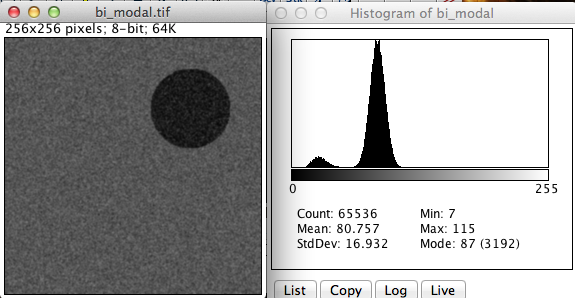
\includegraphics[width=6cm]{images/histogramme_bi_modal}
\end{center}
	\caption{\`A gauche une image bi-modal et \`a droite sont histogramme}
	\label{histo_bi_modal}
\end{figure}

Mais les composantes verte des images que l'on poss\`ede sont tri-modal c'est \`a dire qu'il y a trois niveaux de gris distinct. On a donc adapt\'e la m\'ethode d'Otsu pour trouver deux seuils s\'eparant les trois niveaux de gris. Ensuite on applique un algorithme simple pour "trinaris\'e" cette image. 

Les  ~Fig.~\ref{4_classe_gris_vert} et ~Fig.~\ref{6_classe_gris_vert} sont le r\'esultat de cette m\'ethode sur les ~Fig.~\ref{4_classe} et ~Fig.~\ref{6_classe}

\begin{figure}
\begin{center}
	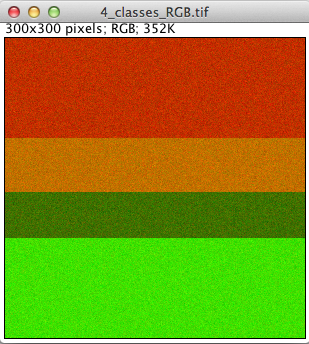
\includegraphics[width=4cm]{images/4_classe}
\end{center}
	\caption{image \emph{4\_classe\_RGB.tif}}
	\label{4_classe}
\end{figure}

\begin{figure}
\begin{center}
	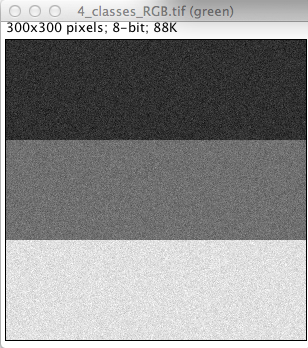
\includegraphics[width=4cm]{images/4_classe_vert}
	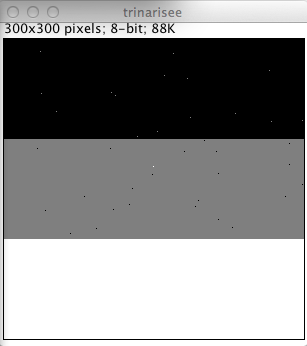
\includegraphics[width=4cm]{images/4_classe_trinaire}
\end{center}
	\caption{\`A gauche la composante verte de l'image \ref{4_classe} et \`a droite le seuillage de celle-ci par la m\'ethode d'Otsu tri-modal}
	\label{4_classe_gris_vert}
\end{figure}

\begin{figure}
\begin{center}
	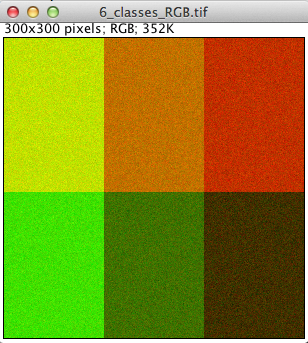
\includegraphics[width=4cm]{images/6_classe}
\end{center}
	\caption{image \emph{6\_classe\_RGB.tif}}
	\label{6_classe}
\end{figure}

\begin{figure}
\begin{center}
	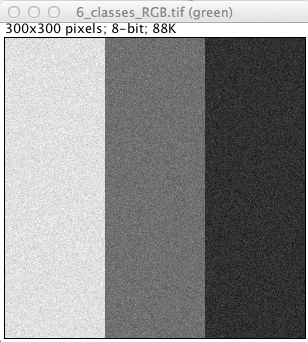
\includegraphics[width=4cm]{images/6_classe_vert}
	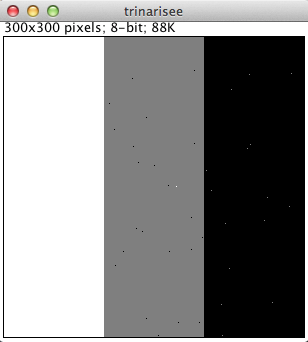
\includegraphics[width=4cm]{images/6_classe_trinaire}
\end{center}
	\caption{\`A gauche la composante verte de l'image \ref{6_classe} et \`a droite le seuillage de celle-ci par la m\'ethode d'Otsu tri-modal}
	\label{6_classe_gris_vert}
\end{figure}

\newpage

%%%%%%%%%%%%%%%%%%%%%%%%%%%%%%%%%%%%%%%%%%%%%
\section{Multi-seuillage d'une image couleur}

Dans la section pr\'ec\'edente nous avons chercher plusieurs seuil au sein d'une m\^eme image. Maintenant on aimerai pouvoir combiner les images en niveau de gris des 3 composantes seuiller afin de recr\'eer une image couleur.

Pour ce faire nous allons seuiller les composantes puis les recombiner. La composante rouge \'etant bi-modal on lui applique la m\'ethode d'Otsu et la composante verte \'etant tri-modal on lui applique la m\'ethode d'Otsu tri-modal. \\

Apr\`es seuillage et combinaison des composante on obtient les ~Fig.~\ref{4_classe_fusion} et Fig.~\ref{6_classe_fusion} \`a partir des ~Fig.~\ref{4_classe} et ~Fig.~\ref{6_classe}

\begin{figure}[ht]
\begin{center}
	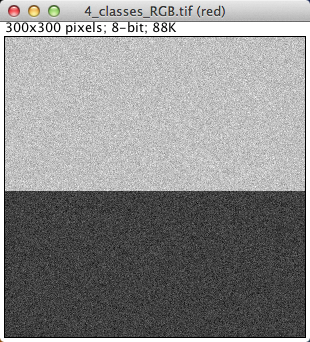
\includegraphics[width=4cm]{images/4_classe_rouge}
	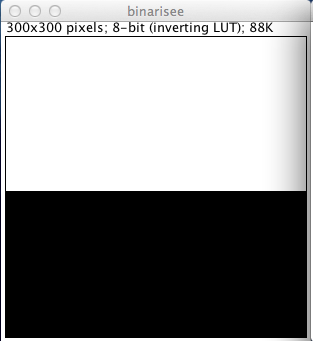
\includegraphics[width=4cm]{images/4_classe_binaire}
\end{center}
	\caption{\`A gauche la composante rouge de l'image \ref{4_classe} et \`a droite le seuillage de celle-ci par la m\'ethode d'Otsu bi-modal}
	\label{4_classe_gris_rouge}
\end{figure}

\begin{figure}
\begin{center}
	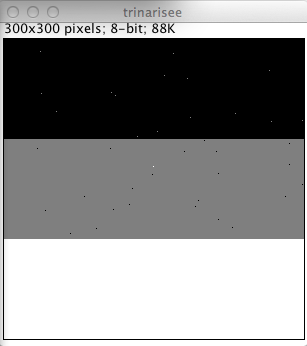
\includegraphics[width=4cm]{images/4_classe_trinaire}
	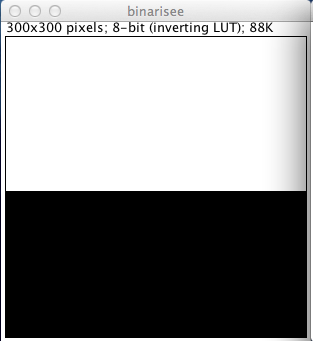
\includegraphics[width=4cm]{images/4_classe_binaire}
	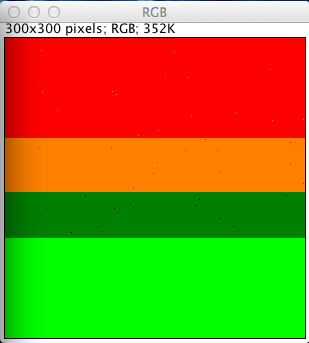
\includegraphics[width=4cm]{images/4_classe_fusion}
\end{center}
	\caption{\`A gauche la composante verte seuill\'e de l'image \ref{4_classe}, au milieu la composante rouge seuill\'e de l'image \ref{4_classe} et \`a droite la fusion des trois composantes seuill\'e (l'image est cod\'e sur les deux composantes verte et rouge donc la composante bleu est noire)}
	\label{4_classe_fusion}
\end{figure}

\begin{figure}
\begin{center}
	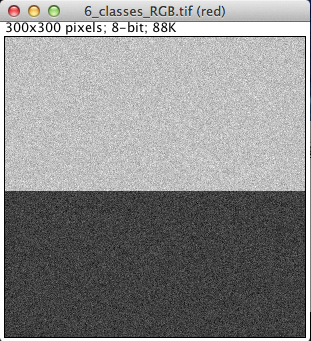
\includegraphics[width=4cm]{images/6_classe_rouge}
	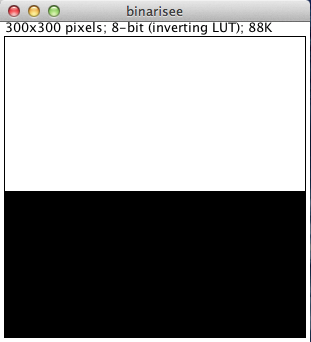
\includegraphics[width=4cm]{images/6_classe_binaire}
\end{center}
	\caption{\`A gauche la composante rouge de l'image \ref{6_classe} et \`a droite le seuillage de celle-ci par la m\'ethode d'Otsu bi-modal}
	\label{6_classe_gris_rouge}
\end{figure}

\begin{figure}
\begin{center}
	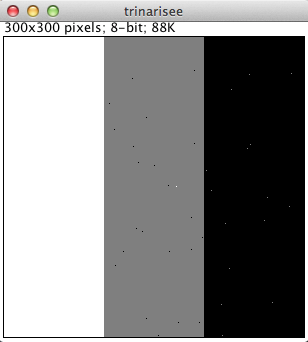
\includegraphics[width=4cm]{images/6_classe_trinaire}
	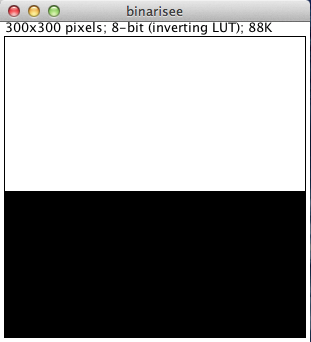
\includegraphics[width=4cm]{images/6_classe_binaire}
	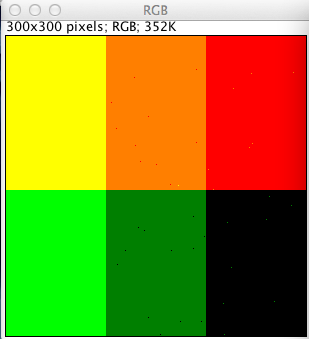
\includegraphics[width=4cm]{images/6_classe_fusion}
\end{center}
	\caption{\`A gauche la composante verte seuill\'e de l'image \ref{6_classe}, au milieu la composante rouge seuill\'e de l'image \ref{6_classe} et \`a droite la fusion des trois composantes seuill\'ees (l'image est cod\'e sur les deux composantes verte et rouge donc la composante bleu est noire)}
	\label{6_classe_fusion}
\end{figure}

\newpage

%%%%%%%%%%%%%%%%%%%%%%%%%%%%%%%%%%%%%%%%%%%%%
\section{Analyse  en composantes principales}

Dans les sections pr\'ec\'edentes on avais la composante verte qui \'etait tri-modal et permettait une segmentation correcte des images.

Si on prend la ~Fig.~\ref{3_classe} et  qu'on lui applique l'algorithme de la partie 2 on obtient la ~Fig.~\ref{3_classe_gris_vert}


\begin{figure}[ht]
\begin{center}
	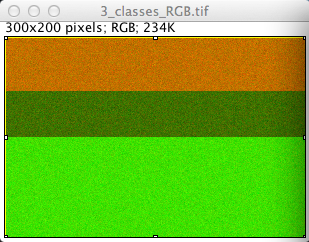
\includegraphics[width=4cm]{images/3_classe}
\end{center}
	\caption{image \emph{3\_classe\_RGB.tif}}
	\label{3_classe}
\end{figure}

\begin{figure}[ht]
\begin{center}
	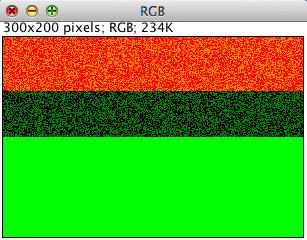
\includegraphics[width=4cm]{images/3_classe_fusion}
\end{center}
	\caption{Image r\'esultant de la fusion des trois composantes seuil\'ees}
	\label{3_classe_gris_vert}
\end{figure}

On voit bien que la segmentation c'est mal effectu\'ee. Les couleurs ne sont pas les bonnes. Le probl\`eme viens du fait que les composantes ne poss\`edent pas assez d'informations pour que la segmentation soit correcte. En effet sur la~Fig.~\ref{3_classe_comp} on voit que chaque composante poss\`ede 2 ou 1 niveau de gris.

\begin{figure}[ht]
\begin{center}
	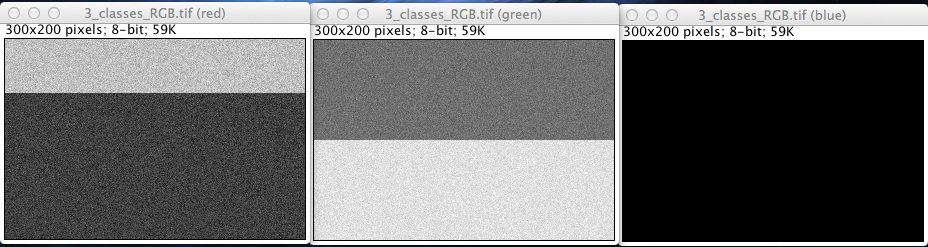
\includegraphics[width=8cm]{images/3_classe_comp}
\end{center}
	\caption{Composantes rouge vert bleu de l'image \ref{3_classe}}
	\label{3_classe_comp}
\end{figure}

Pour pallier \`a ce probl\`eme nous allons utiliser un plugin nomm\'e PCA (Principal Component Analysis). Ce plugin va analyser l'image afin de trouver des composantes qui poss\`edent beaucoup d'informations. En l'appliquant ce plugin sort une pile d'image qui est rang\'ee par ordre d\'ecroissant (plus la composante \`a d'information plus elle est haut sur la pile).

Si on prend la ~Fig.~\ref{3_classe} et qu'on lui applique ce plugin on obtient l'image gauche de la  ~Fig.~\ref{3_classe_comp_prin}. On voit bien trois niveau de gris distinct comparer aux composante vert rouge bleu (\emph{cf.}~Fig.~\ref{3_classe_comp}). 

Ensuite il ne reste qu'\`a appliqu\'e la m\'ethode d'Otsu sur l'image de gauche de la ~Fig.~\ref{3_classe_comp_prin} et on obtient l'image de droite de la~Fig.~\ref{3_classe_comp_prin} qui est correctement seuill\'ee.

\begin{figure}[ht]
\begin{center}
	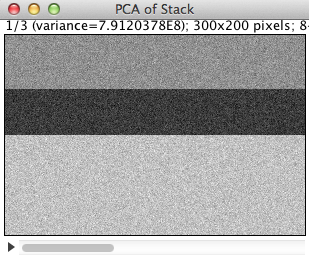
\includegraphics[width=4cm]{images/3_classe_composante}
	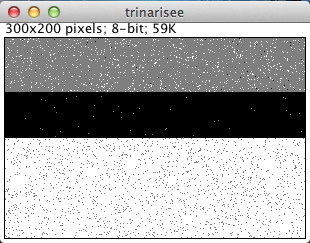
\includegraphics[width=4cm]{images/3_classe_trinaire}
\end{center}
	\caption{\`A gauche la composante principale extraite via le plugin PCA de l'image \ref{3_classe} et \`a droite le seuillage de celle-ci par la m\'ethode d'Otsu tri-modal}
	\label{3_classe_comp_prin}
\end{figure}

\section*{conclusion}

La m\'ethode d'Otsu est une bonne m\'ethode car elle permet de trouver plusieurs seuil au sein d'une m\^eme image. Mais cette m\'ethode \`a ces limites car si les composantes de l'image ne poss\`ede pas beaucoup d'informations alors cette m\'ethode ne trouvera pas de seuil correcte.


\end{document}